\documentclass{beamer}
%\usepackage{beamerarticle}

\usepackage[ngerman]{babel}
\usepackage[utf8]{inputenc}
\usepackage[T1]{fontenc}
\usepackage{tikz}
\usetikzlibrary{positioning, arrows}
\usepackage{listings}
\usepackage{fancybox}
\usepackage{verbatim}

\usepackage{pifont}% http://ctan.org/pkg/pifont
\newcommand{\cmark}{\ding{51}}%
\newcommand{\xmark}{\ding{55}}%

\usetheme{Madrid}
\setbeamercovered{transparent}

\title[SWT-Praktikum]{Pr\"sentationen mit dem Paktet  Beamer}
\author{swp15.gkp}
\date{\today{}}
%\logo{\includegraphics[scale=0.25]{logo}}

\begin{document}

\begin{comment}
\section{Allgemeines}
Im Rahmen des SWT-Praktikums wird ein kartenbasiertes Multiplayerspiel entwickelt, das es ermöglicht, ein an das alte Pacman angelehnte Computerspiel auf einem realen Kartenausschnitt zu spielen. Die entstehenden Highscores werden dann zu den jeweiligen Karten gespeichert, um sich mit anderen Spielern messen zu können.


\section{Produktübersicht}
Der Nutzer kann online über die Spiele Website auf das Programm zugreifen.
%Dabei stehen dem Nutzer ein Suchfeld zum finden der gewünschten Spielumgebung zur Verfügung, es kann auch manuell durch Scrollen über die Karte ein Spielort ausgewählt werden, wobei nur Städte ab einer bestimmten Größe zugelassen sind, damit auf jeden Fall eine spielbare Karte erstellt werden kann und die Highscore vergelichbar bleibt. 
Der Spieler kann durch Scrollen über die Karte einen Spieleort auswählen. Es sind nur bestimmte Orte als Spielort zugelassen, um eine Vergleichbarkeit zu gewährleisten.
Hat man den Ort ausgewählt, wird das Spielfeld erzeugt und man kann ein neues Spiel beginnen. 
Man kann den Pucman nun mit Hilfe der Pfeiltasten steuern.
Ziel des Spiels ist es den Pucman über die Karte zu steuern und die Kekse, die auf der Karte verteilt liegen, zu fressen. 

An dieser Aufgabe will den Spieler der Geist hindern, der sich auch über das Spielfeld bewegt und Pucman fressen kann. Frisst ein Geist den Spieler, so wird %dieser auf den Startpunkt zurückgesetzt und 
die Anzahl seiner Leben wird um eins verringert.
%Es gibt unterschiedliche Geister, die durch ihr aussehen unterschieden werden können und sich anhand verschiedener Logiken bewegen. 
Falls keine Leben mehr übrig sind, wird das Spiel beendet und die erreichte Highscore zusammen mit der Karten URI und dem Namen des Spielers abgespeichert.
Während des Spielens werden die Möglichkeiten zur Veränderung der Kartenansicht deaktiviert. 
Das Spielgeschehen ist durch einen Soundtrack unterlegt, der eine funktionale und inhaltliche Verbindung zwischen Bild und Ton generiert.
Desweiteren werden für das Spiel wichtige Informationen wie aktueller Highscore, die verbleibende Anzahl an Leben und die Möglichkeit, direkt auf die Website des Spiels zugreifen zu können, angezeigt.
\clearpage
\section{Grundsätzliche Struktur- und Entwurfsprinzipien}
Als grundsätzliche Programmiersprache haben wir uns für Java-Script entschieden, wobei der Java-Scriptcode von einer HTML-Seite aufgerufen wird. Desweiteren benutzen wir Phaser als Gameframework.
Ein Teil der Software wurde mithilfe von Funktionen aus der Java-Script Bibliothek JQuery geschrieben, da diese eine intuitive Herangehensweise bietet und für uns verständlicher als klassiches JavaScript ist.
Die von uns umgesetzte Web-Anwendung basiert auf einer Client-Server Architektur. Wir arbeiten mit einem HTML-Server auf dem die Daten liegen, die vom Client abgefragt und an diesen übertragen werden. Diese Daten beinhalten auch den Gameblock, der dann vom Client ausgeführt wird. Außerdem gibt es noch ein Map-Modul, welches das Level aus den Geo-Daten erstellt, die mithilfe der Overpass API von OpenStreetMaps bezogen werden. Dazu kommt das Highscore-Modul, welches für die Verwaltung der Highscores verantwortlich ist.
Desweiteren kommt noch ein Datenserver hinzu, der die Highscores unter Verwendung eines Triplestores speichert.\\
\begin{figure}[htb]
  \centering
  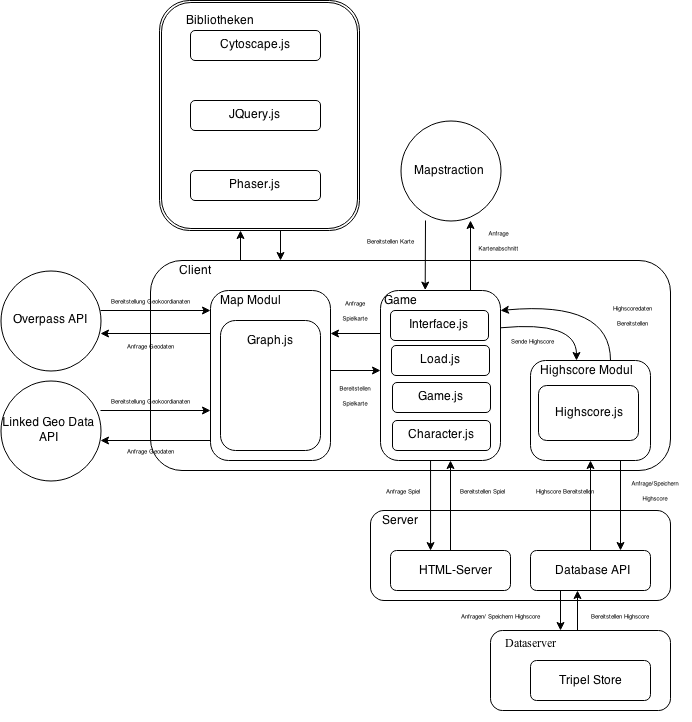
\includegraphics[scale=0.6]{dia_2.png}
\caption{Architekur}
  \label{arch}
\end{figure} 
\section{Struktur- und Entwurfsprinzipien der einzelnen Pakete}
\subsection{Client}
\section{Datenmodell}
Siehe Abbildung \ref{arch}.\bigskip

Beschreibung zu Abbildung \ref{arch}: \\
$A \xlongrightarrow{\text{Datenfluß}} B $ beschreibt den Datenfluss von A nach B, wobei A und B Module der Software sind.
\clearpage
\end{comment}




\begin{frame}
\center \huge \textbf{Kartenbasiertes Multiplayerspiel} \\
\center \huge \textbf{P U C M A N}
\end{frame}

\begin{frame}{Überblick}
\begin{itemize}
\item Produktübersicht
\item Grundsätliche Struktur- und Entwurfsprinzipien
\begin{itemize}
\item Server
\item Client
\begin{itemize}
\item Map-Modul
\item Game-Modul
\item Highscore-Modul
\end{itemize}
\item Bibliotheken
\end{itemize}
\item Testkonzept
\item Erweiterbarkeit
\item Das Projekt im Netz
\end{itemize}
\end{frame}

\begin{frame}{Übersicht}
\begin{figure}[htb]
  \centering
  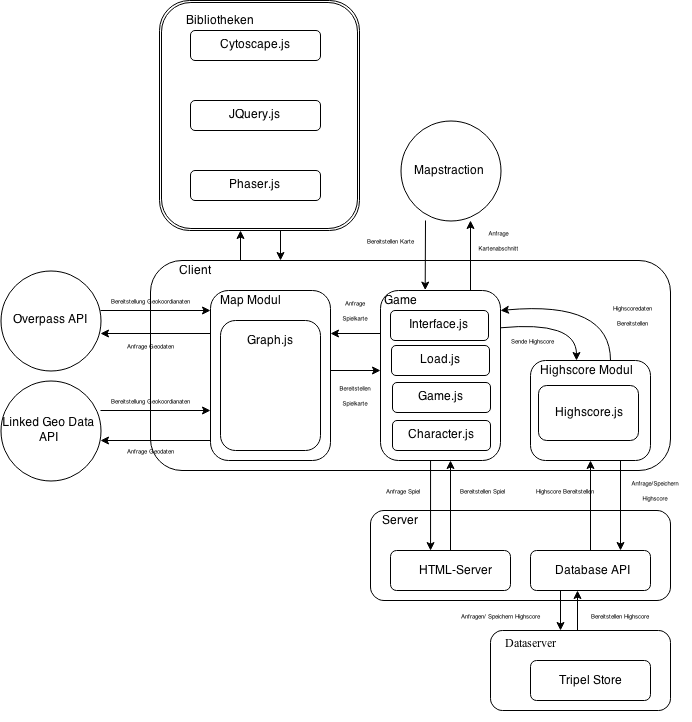
\includegraphics[scale=0.3]{dia_2.png}
\caption{Architekur}
  \label{arch}
\end{figure} 
\end{frame}


\begin{frame}{Map-Modul}
%Die Linked GeoData API extrahiert aus OpenStreetMap die Geo-Daten für das Erstellen der Hintergrundkarte in Abhänigkeit vom gewählten Ort.\\
\begin{itemize}
\item Overpass API extrahiert die Geo-Daten aus OpenStreetMap
\item Vorselektierung durch eine angepasste Query 
\item nur Straßen aus dem Browser Fenster
\end{itemize}
\end{frame}


\begin{frame}{Map-Modul}
\begin{itemize}
\item Anfrage $\Rightarrow$ GeoJson
\item $\Rightarrow$ Cytoscape Graph
\item $\Rightarrow$ Knoten mit Geokoordinaten $\rightarrow$ Pixel

\end{itemize}
\end{frame}


\begin{frame}{Map-Modul}
\begin{itemize}
\item Sackgassen löschen
\item Sternkreuzungen berücksichtigen
\item größter zusammenhängender Teilgraph
\end{itemize}
\end{frame}

\begin{frame}{Map-Modul}
\begin{itemize}
\item Interpolation zwischewn den Knoten um Pixel zu setzen
\end{itemize}
\textbf{Problem:}\\
Die flüssige Bewegung ist leider nicht immer gegeben, da die ausgeführten Funktionen teilweise sehr Rechenaufwändig sind.
Bei alten CPUs (z.B. einem Doppelkernprozessor) läuft das Spiel langsamer, als auf einem neuwertigen i7-Prozessor.

\end{frame}
\begin{frame}
\begin{figure}[htbp] 
  \centering
     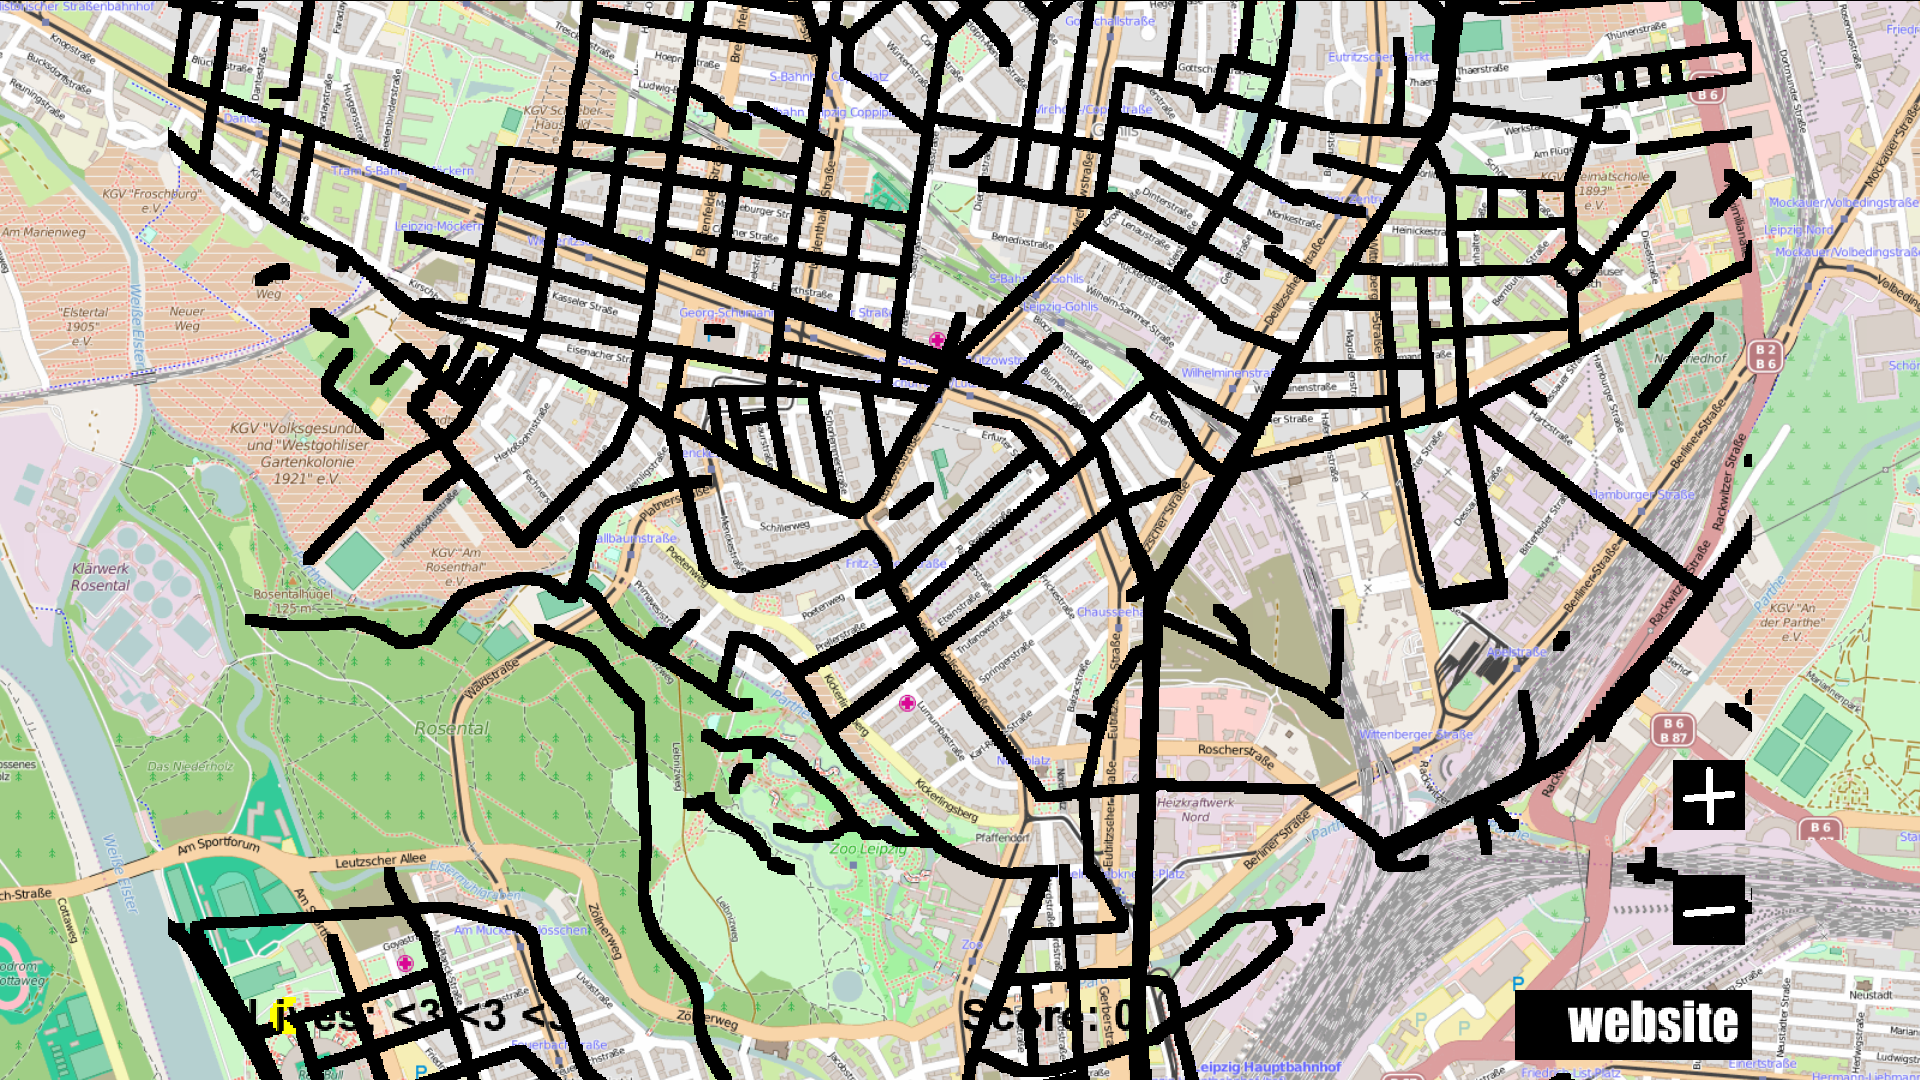
\includegraphics[width=1\textwidth]{03.png}
 % \caption{Erstes Bild}
 % \label{fig:Bild1}
\end{figure}

\end{frame}
\begin{frame}
\begin{figure}[htbp] 
  \centering
     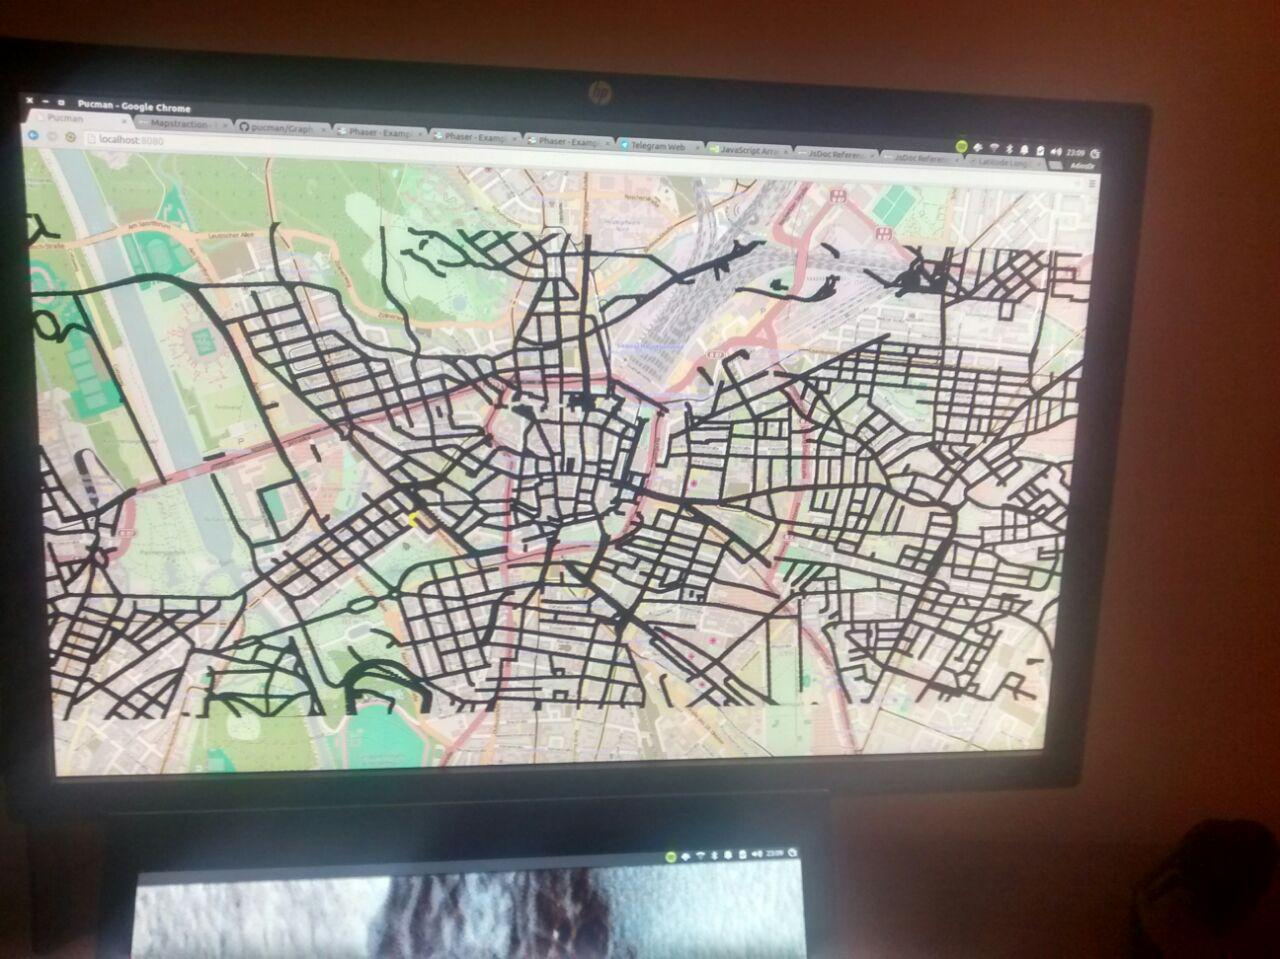
\includegraphics[width=1\textwidth]{05.jpg}
  %\caption{Erstes Bild}
  %\label{fig:Bild1}
\end{figure}

\end{frame}

\begin{frame}
\begin{figure}[htbp] 
  \centering
     
\includegraphics[width=1\textwidth]{06.jpg}
  %\caption{Erstes Bild}
  %\label{fig:Bild1}
\end{figure}

\end{frame}
\begin{frame}
\begin{figure}[htbp] 
  \centering
     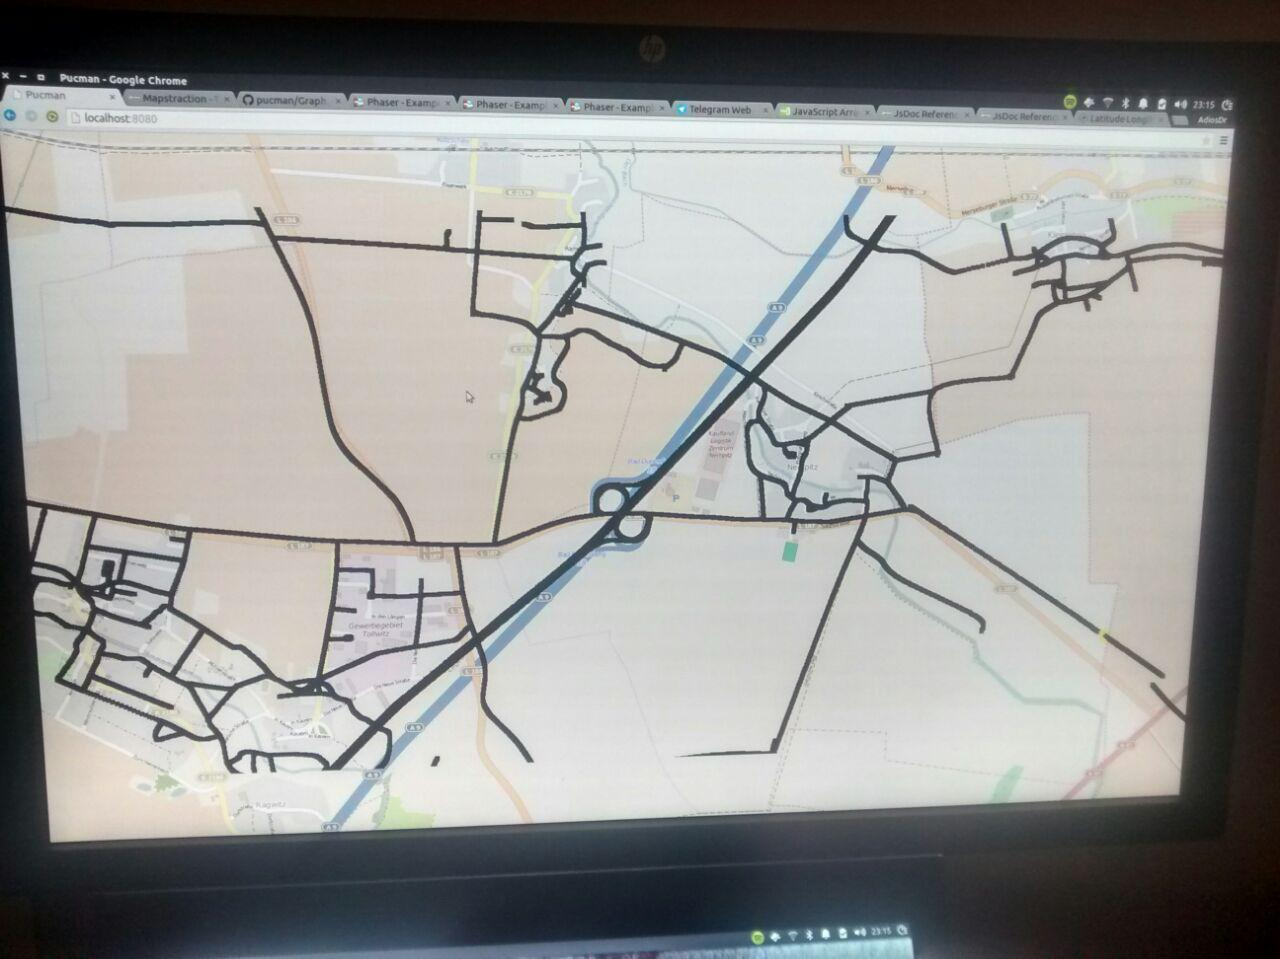
\includegraphics[width=1\textwidth]{07.jpg}
  %\label{fig:Bild1}
\end{figure}

\end{frame}

\begin{frame}
\begin{figure}[htbp] 
  \centering
     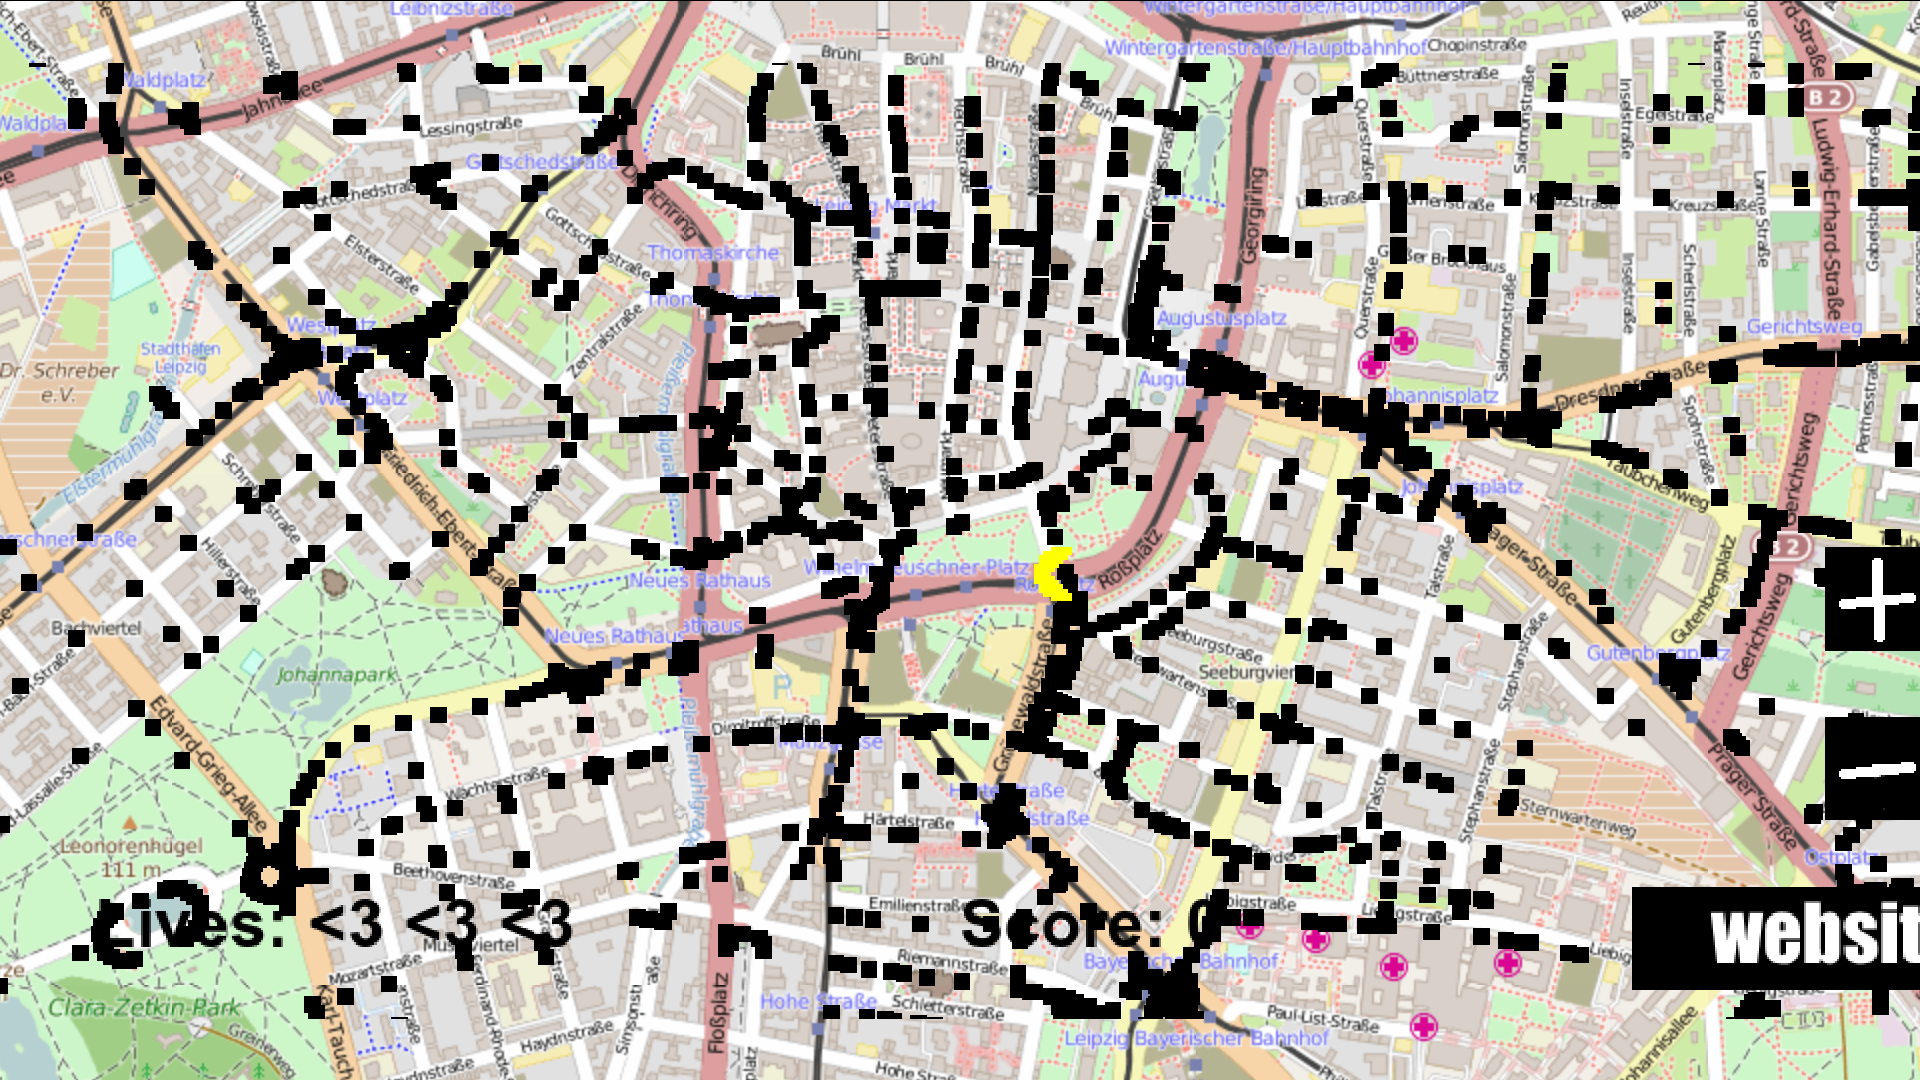
\includegraphics[width=1\textwidth]{04.png}
  %\caption{Erstes Bild}
  %\label{fig:Bild1}
\end{figure}

\end{frame}


\begin{frame}
\begin{figure}[htbp] 
  \centering
     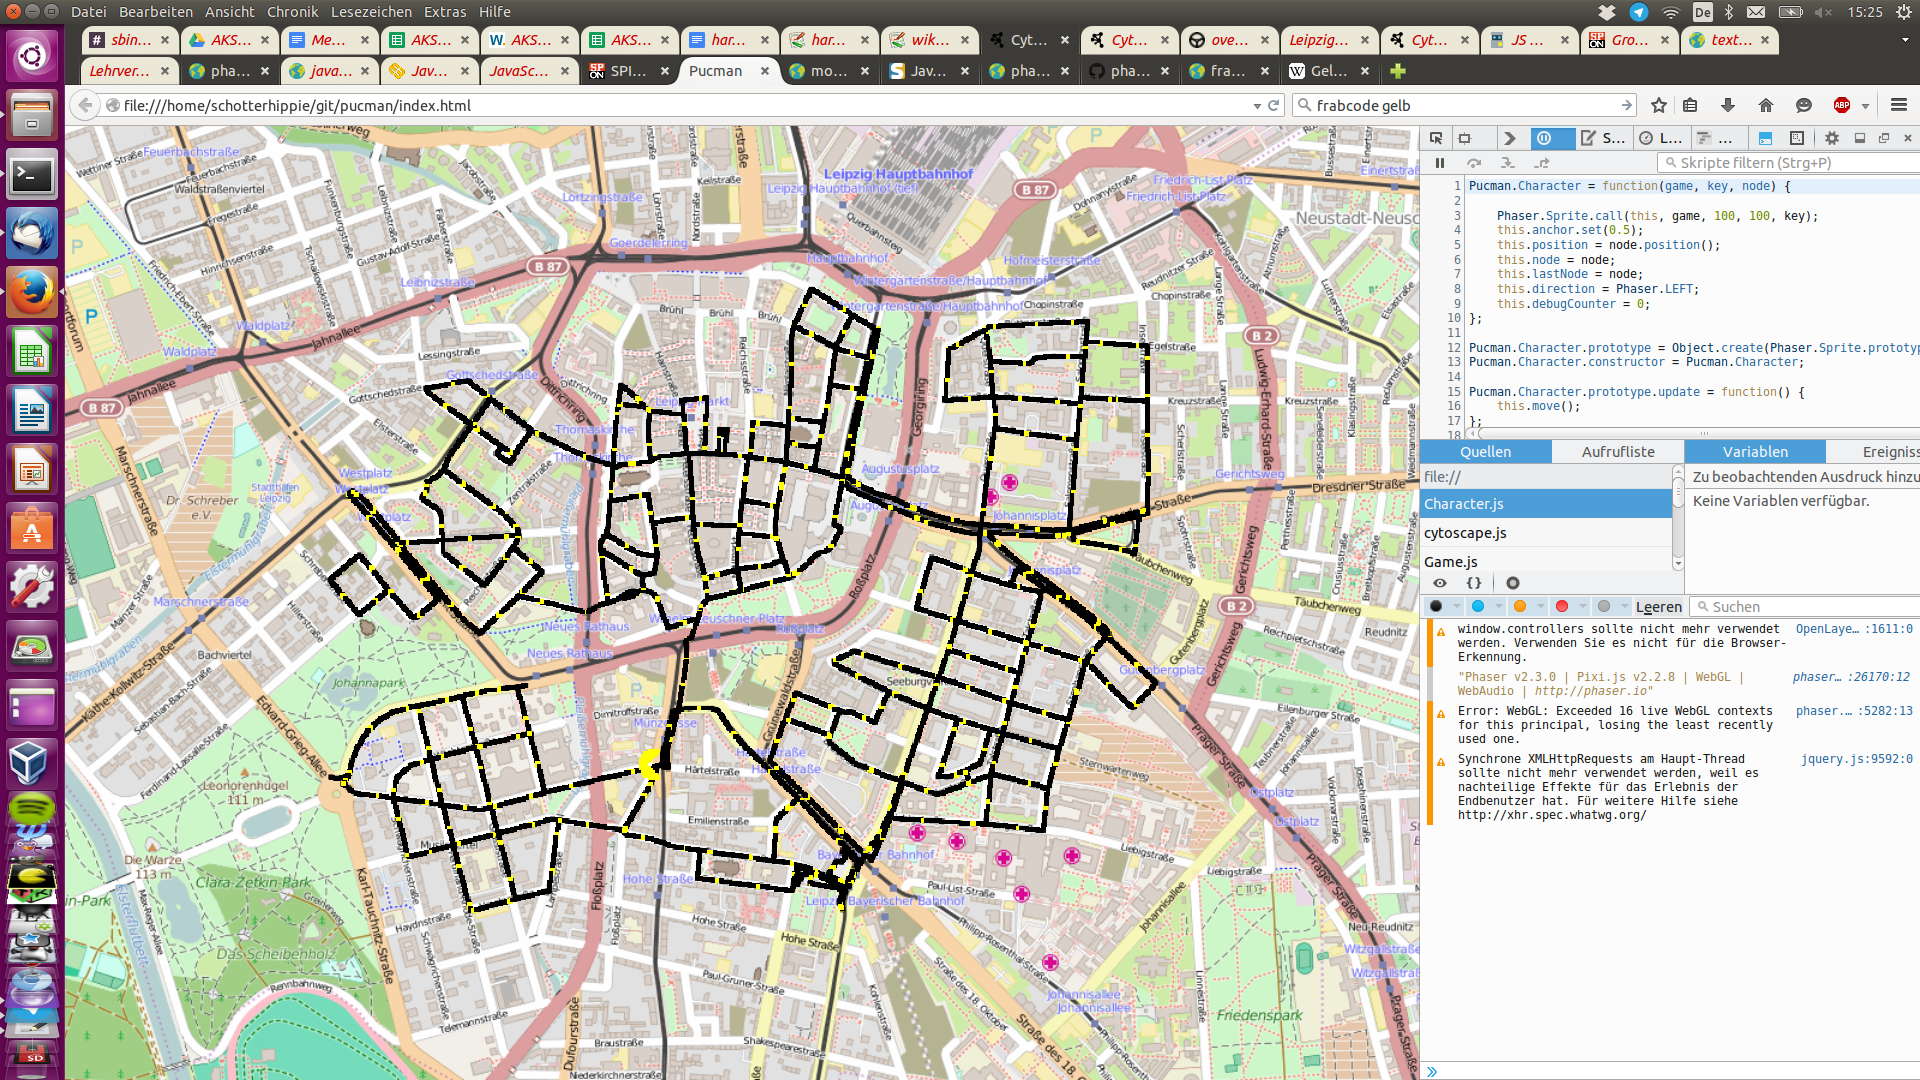
\includegraphics[width=1\textwidth]{01.png}
  %\caption{Erstes Bild}
  %\label{fig:Bild1}
\end{figure}
\end{frame}

\begin{frame}
\begin{figure}[htbp] 
  \centering
     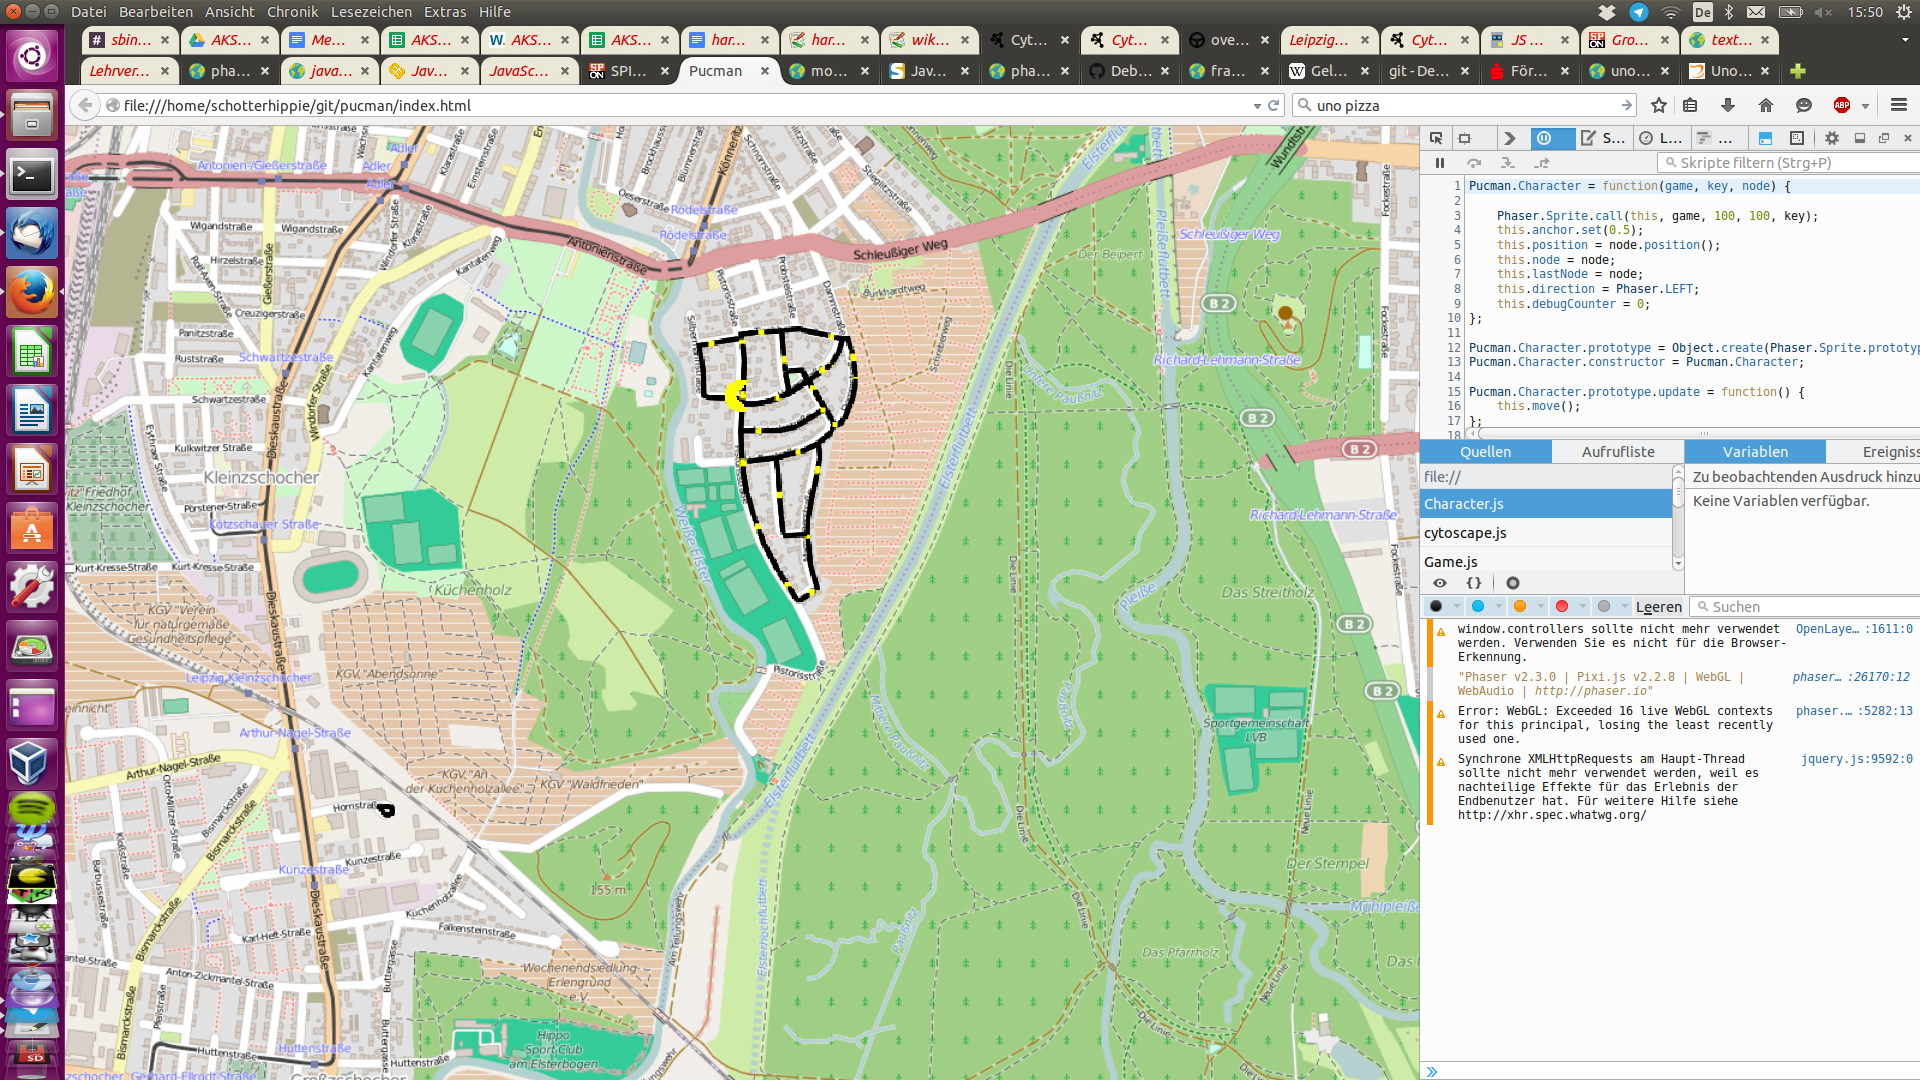
\includegraphics[width=1\textwidth]{02.png}
  %\caption{Erstes Bild}
  %\label{fig:Bild1}
\end{figure}

\end{frame}

\begin{frame}{Game-Modul}

\begin{itemize}
\item Phaser
\begin{itemize}
\item Eingabe- und Ausgabeverarbeitung 
\item Gameloop
\end{itemize}
\end{itemize}
Die Update-Methode enthält: Tastatur- und Mauseingabe, Bewegung, Kollisionserkennung, etc. \\

Die Render-Methode enthält: Anzeige aller Sprites an den neuen Positionen, Hintergrund animieren, etc. \\
\end{frame}
\begin{frame}{Game-Modul}

{\flushleft \textbf{Interface.js:}} 
\begin{itemize}
\item Schnittstelle zum Benutzer
\item Anzeigen, Knöpfe, etc.
\end{itemize}
{\flushleft \textbf{Load.js:}}
\begin{itemize}
\item Ladescreen
\end{itemize}
{\flushleft \textbf{Game.js:}}
\begin{itemize}
\item Gameloop
\end{itemize}
{\flushleft\textbf{Character.js:}}
\begin{itemize}
\item Spielfigur
\end{itemize}
\end{frame}


\begin{frame}{Highscore-Modul}
\begin{itemize}
\item Verwaltet die Highscores der Spieler
\item Anfragen an den Server zum Triplestore
\item SPARQL Queries - Anfrage
\item SPARQL Update Methoden - Einpflegen
\end{itemize}
\end{frame}


\begin{frame}{Bibliotheken}
\textbf{Cytoscape.js:}
\begin{itemize}
\item Graphalgorithmen
\end{itemize} 
\textbf{JQuery.js:} 
\begin{itemize}
\item Vereinfacht den Umgang mit verschiedenen aufgetretenen Problemen 
\end{itemize}
\textbf{Phaser.js}
\begin{itemize}
\item Gameframework
\item Eingabe- und Ausgabeverarbeitung etc.
\end{itemize}
\end{frame}
\begin{frame}{Testkonzept}
\begin{itemize}
\item Github Test-Workflows
\end{itemize}Dabei werden die angegebenen Eingaben getätigt und die Reaktion der Software mit der erwarteten Ausgabe verglichen. Sollten dabei Abweichungen auftreten, gilt der Test als nicht bestanden.
\end{frame}
\begin{frame}{Testumgebungen}
\small
\begin{enumerate}
\item OS: Ubuntu 15.04 \\
Kernel: Linux version 3.19.0-18-generic \\
CPU: Intel(R) Core(TM) i7-4712MQ CPU @ 2.30GHz \\
RAM: 8GiB \\
Firefox 30.0 \\
\textbf{Resultat: Läuft flüssig.}
\item OS: Ubuntu 15.04\\
Kernel: Linux version 3.19.0-18-generic \\ 
CPU: Intel Core i5-2520M CPU @ 2.50GHz x 4 \\
RAM: 7,7 GiB \\
Chrome 42.0.2311.90 (64-bit) \\
\textbf{Resultat: Läuft flüssig bei 30\% Auslastung mit 15\% Idle.}
\item OS: Arch Linux \\
Kernel: x86\_64 Linux 4.0.3-1-ARCH \\
CPU: Intel Core2 Duo CPU T7300 @ 2.001GHz \\
RAM: 3883MB \\
Firefox 38.0.1 \\
\textbf{Resultat: Läuft eher langsam, ein Kern voll ausgelastet.}
\end{enumerate}
\end{frame}

\begin{frame}{Erweiterbarkeit}
\normalsize
\begin{itemize}
\item Modularisierung von Vorteil
\item z.B. Mapstraction
\item Geister KI, semantische Daten
\end{itemize}
\end{frame}
\begin{frame}{Das Projekt im Netz}
\begin{itemize}
\item Projekt Website: \url{http://pcai042.informatik.uni-leipzig.de/~swp15-gkp/} 
\item Source-Code: \url{https://github.com/GKP15/pucman}
\end{itemize}

\end{frame}
\begin{frame}{Struktur des Source-Codes:}
\textbf{/lib} \\
Hier liegen die Bibliotheken, die wir benötigt haben, wie Phaser, Cytoscape, etc. \par\bigskip
{\flushleft \textbf{/rdf}} \\
Daten für den Triplestore. \par\bigskip
{\flushleft \textbf{/resources}} \\
Bilder, Musik, etc. \par\bigskip
{\flushleft \textbf{/src}} \\
Die einzelnen Module für das Spiel, als Java-Script Code. \par\bigskip
{\flushleft \textbf{/}} \\
Die Html-Dateien, Config-Dateien, etc.  

\end{frame}






\begin{frame}
\Huge \center \textbf{F R A G E N ?}
\end{frame}
\end{document}